\section{Background: Web Performance Metrics \& Tools}

\begin{frame}
    \frametitle{Important Metrics}
	Three of the most common metrics for web performance in surveyed papers:
	\begin{enumerate}
	  \item \textbf{Load Time} - The time required for loading a web page correlates strongly with user experience \cite{6263888}. Page Load Time (PLT), defined as the time until the onLoad event, is most often used to measure page load times; there are, however, a number of other metrics.
	  \item \textbf{Object Size} - Object size normally reflects the encoded size (i.e. the count of bytes transferred over the network) but can also reflect the decoded (i.e. decompressed) number of bytes. Byte Index refers to the integral of the total sizes of objects loaded over time and is an important metric for objects \cite{10.1145/2940136.2940138}.
	  \item \textbf{Object Count} - Calculating a count of the initial objects can be done using objects in the DOM or HTTP request-response pairs.
	\end{enumerate}
\end{frame}

\begin{frame}
    \frametitle{Metric Definition: Load Time}
	\begin{figure}
			\centering
			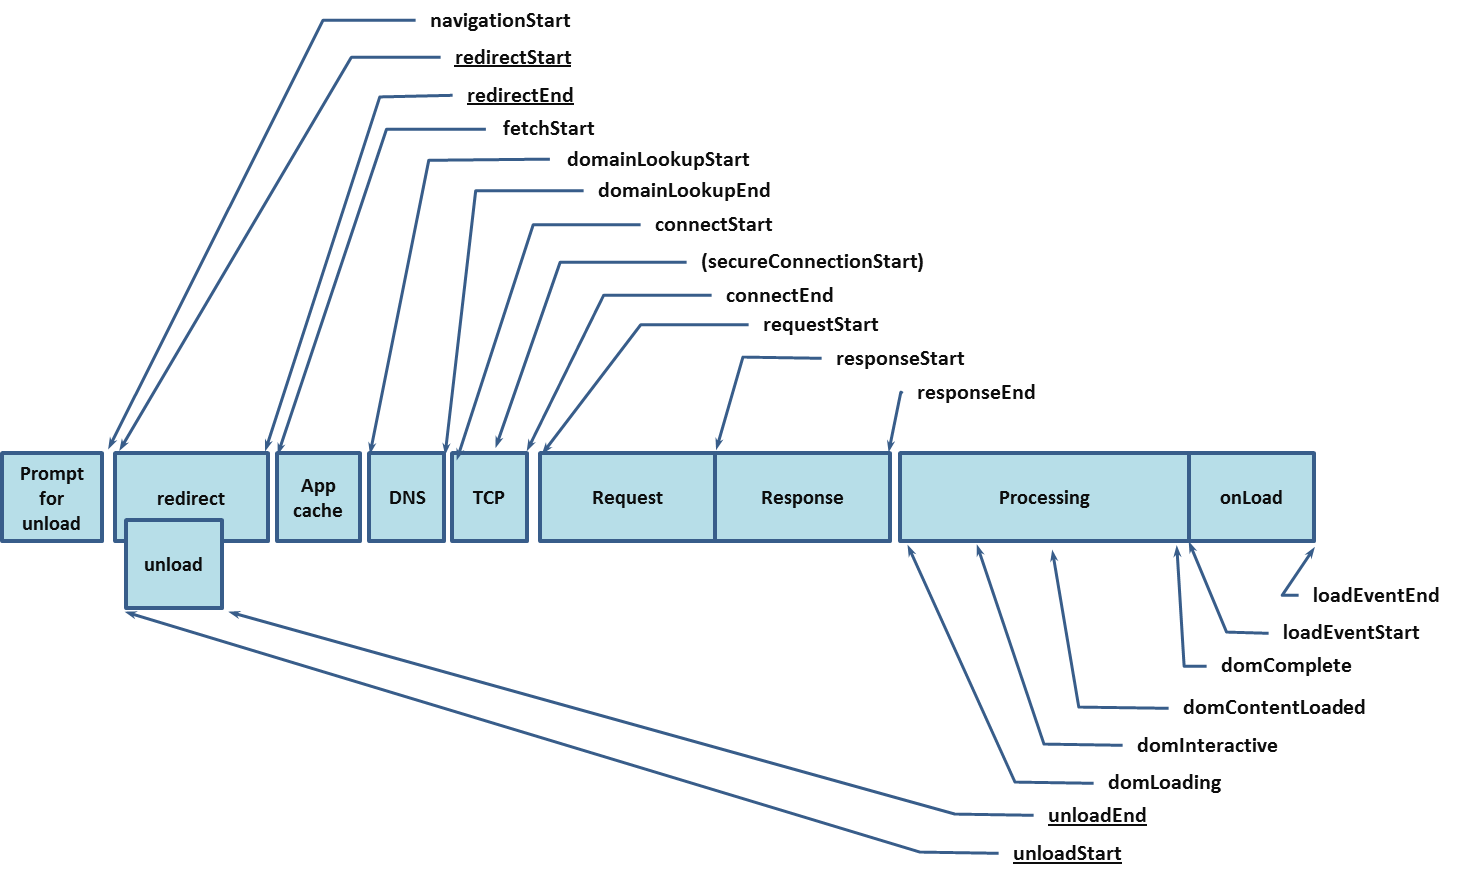
\includegraphics[width=.7\textwidth,keepaspectratio]{pics/timing-overview.png}
		\caption{Overview of Timing Events \cite{timing_2012}}
		\label{fig:timing_event}
	\end{figure}
Although Page Load Time (PLT), i.e. the onLoad event, is most often used to measure page load times, there are a number of other metrics (e.g. Time To First Paint (TTFP) and Above The Fold Time (AFT)).
	
\end{frame}

\begin{frame}
    \frametitle{Data Sources}
    The three most common data sources used in surveyed papers:
	\begin{enumerate}
	  \item \textbf{Navigation Timings} - Standardized API for navigation timings - load times based on browser events \cite{timing_2012}
	  \item \textbf{Resource Timings} -  Standardized API for resource timings and encoded / decoded body size of each object \cite{w3c_2020}
	  \item \textbf{HTTP Archive (HAR) Files} -  Encoded / decoded body size of each object \cite{har_format_2012}
	\end{enumerate}
	 $\boldsymbol{\rightarrow}$ Metrics can vary greatly in definition and source \cite{10.1007/978-3-030-15986-3_19}.
\end{frame}